\section{Recurrencias Lineales con coeficientes constantes}

Una relación de recurrencia lineal de orden $r$ con coeficientes constantes es una recurrencia del tipo:
\begin{align}\label{1}
c_{0}x_{n}+c_{1}x_{n-1}+\cdots+c_{r}x_{n-r}=h_{n},\forall n\geq r,
\end{align}
donde $c_{0},c_{1},\ldots,c_{r}$ son constantes reales o complejas, con $c_{0}$ y $c_{r}$ ambos diferentes de cero y $(h_{n})_{n\geq r}$ es una sucesión de números reales o complejos llamado sucesión de términos no homogéneos de la recurrencia. La recurrencia es llamada homogénea si la sucesión de términos no homogéneos es una sucesión nula, no homogénea si $h\neq0 $ para algún $n$. La relación de recurrencia:
\begin{align}\label{2}
c_{0}x_{n}+c_{1}x_{n-1}+\cdots+c_{r}x_{n-r}=0,\forall n\geq r,
\end{align}
es llamada la recurrencia homogénea asociada, o la parte homogénea de la recurrencia \eqref{1}. Como nosotros ya hemos notado, la recurrencia:
\begin{equation*}
c_{0}x_{n}+c_{1}x_{n-1}+\cdots+c_{r}x_{n-r}=h_{n},\forall n\geq r,
\end{equation*}
puede ser escrito equivalentemente como
\begin{equation*}
c_{0}x_{n+r}+c_{1}x_{n+(r-1)}+\cdots+c_{r}x_{n}=h_{n+r},\forall n\geq 0.
\end{equation*}
Se puede utilizar cualquiera de las formas presentadas.

\begin{remark}
	Cada $r$-secuencia de valores asignados a las $r$ incógnitas desconocidas de la relación de recurrencia
	\begin{equation*}
	c_{0}x_{n}+c_{1}x_{n-1}+\cdots+c_{r}x_{n-r}=h_{n},\forall n\geq r,
	\end{equation*}
	determina de forma única una solución. Al resolver una relación de recurrencia lineal, el siguiente principio es fundamental importancia.
\end{remark}

\begin{proposition}[Principio de superposición]\index{Principio de superposición}
	Sean ${(u_{n})}_{n}$, ${(V_{n})}_{n}$ respectivamente las soluciones de las relaciones de recurrencia lineal.
	\begin{align*}
	c_{0}x_{n}+c_{1}x_{n-1}+\cdots+c_{r}x_{n-r}&=h_{n},\quad n\geq r
	\intertext{y}
	c_{0}x_{n}+c_{1}x_{n-1}+\cdots+c_{r}x_{n-r}&=k_{n},\quad n\geq r,
	\end{align*}
	con partes homogéneas iguales y secuencias de términos no homogéneos $(h_{n})_{n}$ y $(k_{n})_{n}$. Para cualquier par de constantes $A$ y $B$, la sucesión $(Av_{n}+Bv_{n})_{n}$ es una solución de la relación de recurrencia. \[ c_{0}x_{n}+c_{1}x_{n-1}+\cdots+c_{r}x_{n-r}=Ah_{n}+Bk_{n}. \] La solución general de la relación de recurrencia
	\begin{equation}\label{eq:super}
	c_{0}x_{n}+c_{1}x_{n-1}+\cdots+c_{r}x_{n-r}=h_{n},\quad n\geq r.
	\end{equation}
\end{proposition}

\begin{proof}\leavevmode
	\begin{enumerate}
		\item Uno tiene fácilmente
		\begin{equation*}
		\begin{split}
		&c_{0}(Au_{n}+Bv_{n})+c_{1}(Au_{n-1}+Bv_{n-1})+\cdots+c_{r}(Au_{n-r}+Bv_{n-r})=\\
		&\phantom{c_{0}(Au_n+}=A(c_{0}u_{n}+c_{1}u_{n-1}+\cdots+c_{r}u_{n-r})+B(c_{0}v_{n}+c_{1}v_{n-i}+\cdots+c_{r}v_{n-r})\\
		&\phantom{c_{0}(Au_n+}=Ah_{n}+Bk_{n}.
		\end{split}
		\end{equation*}
		\item Sea $(u_{n})_{n}$ una solución particular de \eqref{eq:super}. Por el punto previo nosotros conocemos que $(v_{n})_{n}=(u_{n})_{n}+(v_{n}-u_{n})_{n}$ es una solución de \eqref{eq:super} si y solo si $v_{n}-u_{n}$ es una solución de la recurrencia homogénea asociada. Por lo tanto cada solución de \eqref{eq:super} es obtenida añadiendo una solución de la  recurrencia homogénea asociada para $(u_{n})_{n}$.
	\end{enumerate}
\end{proof}

\section{Relación de recurrencia lineal con homogénea con coeficientes constantes}

La sucesión nula es una solución de cualquier relación de recurrencia lineal. La estructura de la solución general de una relación de recurrencia lineal homogénea corresponde a la estructura de la solución general de un sistema de ecuaciones lineales homogéneas.
\begin{proposition}[Teorema principal]
	Considere la relación de recurrencia lineal homogénea de orden $r$:
	\begin{equation}\label{eq:homo}
	c_{0}x_{n}+c_{1}x_{n-1}+\cdots+c_{r}x_{n-r}=0,\quad n\geq r\quad\left(c_{0}c_{r}\neq0\right)
	\end{equation}
	\begin{enumerate}
		\item Cualquier combinación lineal de soluciones de \eqref{eq:homo} es de nuevo una solución de \eqref{eq:homo}.
		\item Existe $r$ soluciones de \eqref{eq:homo} tal que cualquier otra solución de \eqref{eq:homo} puede ser expresado únicamente como su combinación lineal.
	\end{enumerate}
\end{proposition}

\begin{proof}\leavevmode
	\begin{enumerate}
		\item Esto sigue inmediatamente por el ``Principio de Superposición''.
		\item Para todo $i\in\left\{0,\ldots,r-1 \right\}$ sea $\left(u^{i}_{n}\right)_{n}$ la solución de \eqref{eq:homo} con $r$--sucesión de valores iniciales iguales a $0$ para índices $j\neq i$, iguales a $1$ en índices $i$, es decir: \[ u^{i}_{j}=0\text{ si }j\neq i,\quad u^{i}_{i}=1\quad j\in\left\{0,\ldots,r-1 \right\}. \]
		Consideramos ahora alguna solución $(a_{n})_{n}$ de \eqref{eq:homo}; la combinación lineal \[ a_{0}{\left(u^{0}_{n}\right)}_{n}+a_{1}{\left(u^{1}_{n}\right)}_{n}+\cdots+a_{r-1}(u^{r-1}_{n})_{n}, \]	es una solución de \eqref{eq:homo} con secuencia de datos iniciales $\left(a_{0},\ldots,a_{r-1}\right)$. Ya que la sucesión de valores iniciales determinan la solución de una relación de recurrencia, uno tiene \[ {\left(a_{n}\right)}_{n}=a_{0}\left(u^{0}_{n}\right)_{n}+a_{1}\left(u^{1}_{n}\right)_{n}+\cdots+a_{r-1}\left(u^{r-1}_{n}\right)_{n}. \]
	\end{enumerate}
\end{proof}

\begin{definition}[Polinomio característico]\index{Relación de recurrencia!polinomio característico}
	Definimos el \emph{polinomio característico} de una relación de recurrencia con coeficientes constantes de orden $r$ de la siguiente manera: \[ c_{0}x_{n}+c_{1}x_{n-1}+\cdots+c_{r}x_{n-r}=h_{n},\quad n\geq r\left(c_{0}c_{r}\neq0\right), \] para el polinomio de grado $r$: \[ P(X)\coloneqq c_{0}X^{r}+c_{1}X^{r-1}+\cdots+c_{r}. \] Cada polinomio de grado $r$ tiene exactamente $r$ raíces complejas contando con su multiplicidad. Vemos ahora que la sucesión de las potencias naturales de una determinada raíz del polinomio característico de una relación de recurrencia lineal es una solución de la correspondiente relación homogénea.
\end{definition}

\begin{proposition}[Raíz del polinomio característico]\index{Relación de recurrencia!polinomio característico!raíz}
	Sea $\lambda\in\mathds{C}$. La sucesión $\left(\lambda^{n}\right)_{n}$ de las potencias de $\lambda$ es una solución de la relación de recurrencia lineal homogénea
	\begin{align}\label{5}
	c_{0}x_{n}+c_{1}x_{n-1}+\cdots+c_{r}x_{n-r}=0,\quad n\leq r \quad (c_{0}c_{r}\neq 0),
	\end{align}
	sii $\lambda$ es una raíz de este polinomio característico.
\end{proposition}

\begin{proof}
	Dado que $c_{r}\neq0$, las raíces del polinomio característico deben ser necesariamente no nulas. Sustituyendo los valores de la sucesión ${\left(\lambda^{n}\right)}_{n}$ en la recurrencia, uno tiene \[ c_{0}x_{n}+c_{1}x_{n-1}+\cdots+c_{r}x_{n-r}=0, \] y dividiendo por $\lambda^{n-r}\neq0$ \[ c_{0}\lambda^{r}+c_{1}\lambda^{r-1}+\cdots+c_{r}=0. \]	Por lo tanto, la sucesión ${\left(\lambda^{n}\right)}_{n}$ es una solución de \eqref{5} sii $\lambda$ es una raíz del polinomio $c_{0}X^{r}+c_{1}X^{r-1}+\cdots+c_{r}$.
\end{proof}

En general, no es fácil encontrar las raíces de un polinomio de grado mayor que dos, aunque uno puede siempre usar un adecuado CAS. El siguiente criterio simple, sin embargo, muestra cómo encontrar las raíces racionales de un polinomio con coeficientes enteros.

\begin{proposition}[Las raíces racionales de un polinomio con coeficientes enteros]
	Sea $P(X)=c_{0}X^{r}+c_{1}X^{r-1}+\cdots+c_{r}$ un polinomio con coeficientes enteros $c_{0}\ldots c_{r}\in\mathds{Z}$, con $c_{0}\neq 0$. Si la fracción $\tfrac{a}{b}$ con $a,b\in\mathds{Z}$ con $\operatorname{mcd}=1$ es una raíz de $P(X)$, luego $a\divides c_{r}$ y $b\divides c_{0}$. En particular, si $c_{0}=\pm1$ las raíces racionales del polinomio $P(X)$ son enteros que dividen a $c_{r}$.
\end{proposition}

\begin{proof}
	Dado $c_{0}\left(\frac{a}{b}\right)^{r}+c_{1}{\left(\frac{a}{b}\right)}^{r-1}+\cdots+c_{r-1}\left(\frac{a}{b}\right)+c_{r}=0$, multiplicado por $b^{r}$ obtenemos: \[ 	c_{0}a^{r}+c_{1}a^{r-1}b+\cdots+c_{r-1}ab^{r-1}+c_{r}b^{r}=0. \] Como $a\divides c_{0}a^{r}+c_{1}a^{r-1}b+\cdots+c_{r-1}ab^{r-1}$, luego tiene que dividir también $c_{r}b^{r}$, y por lo tanto, al no tener $a$ y $b$ factores comunes, $a\divides c_{r}$. Análogamente $b\divides c_{0}a^{r}$ y por lo tanto divide a $c_{0}$.
\end{proof}

\begin{example}[Polinomio característico]
	La recurrencia homogénea de segundo orden: \[ x_{n}=2x_{n-1}-2x_{n-2},\quad n\geq2, \] tiene polinomio característico $X^{2}-2X+2$ cuyas raíces son $\lambda_{1}=1-i$ y $\lambda_{2}=1+i$. Las sucesiones ${\left((1-i)^{n}\right)}_{n}$ y ${\left((1+i)^{n}\right)}_{n} $ son las soluciones bases de la recurrencia. La solución general compleja de la recurrencia es: \[ x_{n}=A_{1}{\left(1-i\right)}^{n}+A_{2}{\left(1+i\right)}^{n},\quad n\geq 0, \] con la variante de $A_{1}$ y $A_{2}$ entre los números complejos. Veamos la solución real general. Uno tiene: \[ \lambda_{1}=1-i=\sqrt{2}\left(\frac{\sqrt{2}}{2}-\frac{\sqrt{2}}{2}i\right)=\sqrt{2}\left(\cos\left(\frac{\pi}{4}\right)-i\sen\left(\frac{\pi}{4}\right)\right) \] y \[ \lambda_{2}=1+i=\overline{\lambda_{1}}=\sqrt{2}\left(\cos\left(\frac{\pi}{4}\right)-i\sen\left(\frac{\pi}{4}\right)\right). \] Luego, las sucesiones ${\left(2^{n/2}\cos\left( \frac{n\pi}{4}\right)\right)}_{n}$ y ${\left(2^{n/2}\sen\left(\frac{n\pi}{4}\right)\right)}_{n}$ son las soluciones base reales de la recurrencia. Por lo tanto, la solución general real de la recurrencia es: \[ x_{n}=A_{1}2^{n/2}\cos\left(\frac{n\pi}{4}\right)+A_{2}2^{n/2}\sen\left(\frac{n\pi}{4}\right),\quad n\geq 0, \] con la variación de $A_{1}$ y $A_{2}$ entre los números reales.
\end{example}

\subsection{Algunos modelos de recurrencias lineales}\label{subsec:models}

Ahora damos una serie de ejemplos que ilustran cómo reducir la solución de un problema en el que la búsqueda de las soluciones de una relación de recurrencia apropiada.

\begin{example}[Número de Catalan]
	El número de Catalan ($C_{n} $) es igual al número de rutas de la esquina inferior izquierda de una rejilla cuadrada de $n\times n$ a la esquina superior derecha si estamos restringidos a viajar solo a la derecha o hacia arriba y si se permite tocar pero no pasar arriba de la diagonal entre la esquina inferior izquierda y la superior derecha. Tal ruta recibe el nombre de \emph{ruta buena}. Se da una relación de recurrencia para los números de Catalan. Las rutas buenas se dividen en clases con base en  la primera vez que tocan la diagonal después de salir de la esquina inferior derecha.Por ejemplo,la ruta en la figura toca la diagonal primero en el punto ($3,3$).Las rutas que tocan la diagonal primero en el punto$(k,k)$ se consideran construidas por un proceso de dos pasos:
	\begin{enumerate}
		\item Primero, se construye la parte de $(0,0)$ a $(k,k)$.
		\item Segundo, se construye la parte de $(k,k)$ a $(n,n)$. Una buena ruta siempre sale de $(0,0)$ moviéndose hacia la derecha a $(1,0)$ y siempre llega a $(k,k)$ moviéndose hacia arriba desde $(k,k-1)$.
		\item Los movimientos de $(1,0)$ a $(k,k-1)$ dan una ruta buena en la rejilla de $(k-1)\times(k-1) $ con esquina en $ (1,0),(1,k-1),(k,k-1)$ y $ (k,0)$. En la figura, se marcaron los puntos $(1,0)$ y $(k,k-1),k=3$, con rombos, y se aisló la subrejilla de $(k-1)\times(k-1)$. Así, hay $C_{k-1}$ rutas de $(0,0)$ a $(k,k)$ que tocan primero a la diagonal en $(k,k)$.
		\item La parte de $(k,k)$ a $(n,n)$ es una buena ruta en la rejilla de $(n-k)\times(n-k)$ con esquinas en $(k,k),(k,n),(n,n)$ y $(n,k)$ (vea la figura). Hay $C_{n-1}$ rutas de este tipo. Por el principio de la multiplicación, hay $C_{k-1}C_{n-k}$ rutas buenas en una rejilla de $n\times n$ que tocan primero la diagonal en $(k,k)$. Las rutas buenas que tocan por primera vez en $(k^{\prime}, k^{\prime}),k\neq k^{\prime}$. Entonces se utiliza el principio de la suma a fin de obtener una relación de recurrencia para el número total de rutas buenas en una rejilla de $n\times n$:
	\end{enumerate}
	\[ C_{n}=\sum_{k=1}^{n}C_{k-1}C_{n-k}. \]
	\begin{figure}[ht!]
		\sidecaption[t]%[ht!]
		\centering
		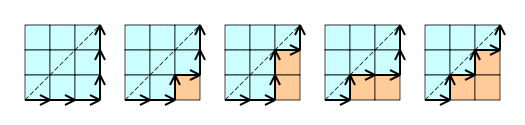
\includegraphics[width=0.4\paperwidth]{./img/catalan}
		\caption{\label{fig:catalan} Retículo de tamaño $\left(k,k\right)$.}
	\end{figure}
\end{example}

\begin{example}[La escalera]
	Un niño decide escalar una escalera con $n\geq 1$ de tal manera que cada paso que él despeja uno o dos de los pasos de la escalera %(vea)
	Encuentre la relación de recurrencia que sirva para calcular el número de diferentes maneras posibles de escalar la escalera.
\end{example}
Usamos la variable desconocida $x_{n}$ para denotar el número de maneras en las cuales el niño puede escalar la escalera de $n\geq1$ pasos. Es fácil de observar que $x_{1}=1$ y $x_{2}=2$ (dos pasos cada uno de longitud uno, o un paso de longitud dos escalones). Ahora sea $n\geq3$: si con el primer paso el niño mueve solo el primer escalón; existen claramente $x_{n-1}$ posibles maneras de escalar los que quedan. Si en cambio con el primer lugar, se suben dos peldaños de escalera.